\chapter{Component Selection and Design}
\justifying
\section[Solar Panels]{Solar Panels}
 TJ Solar Cell 3G30C - Advanced is selected. This cell is a GaInP/GaAs/Ge on Ge substrate triple junction solar cell. The end-of-life version of the 3G30C solar cell offers best EOL-performance
 values. Connected to the EPS via an external bypass diode protection.
 
 Specifications:
 \begin{itemize}
 	\item Average Open Circuit Voltage: 2.7V
 	\item Maximum Power Point Voltage: 2.41V
 	\item Average Short Circuit Current: 520.2 mA
 	\item Maximum Power Point Current: 504.4mA
 \end{itemize}
It has an average efficiency of 29.8\% at 1353 $W/m^{2}$. This solar cell is excellent for space applications. 
\\

Since a CubeSat has six sides and one cell of selected model fits half of a side, a total of 12 cells can be placed.\\ 

Power from a solar panel, P :\\
\hspace*{2cm} $P = P_{i} \times Area \times \eta  \times cos \alpha $ 
\\
 Where, \\
 $P_{i}$ = incident power from sun (1367 W/$m^2$ at Low Earth Orbit)
\\  $\eta$ = conversion efficiency of cell (take 20\% for contingency)
\\  $\alpha$ = angle between normal of cell and incident light (avg: $35^{o} $)\\ \\
Area of solar cell at one face : 0.0032 * 2 = 0.0064 $m^2$\\
\\ \\ Therefore, $P = 1367 W/m^2 \times 0.0064 \times 20  \times cos 35^{o} $ = 1.43W
Assume two faces of CubeSat is lit by sunlight every time except eclipse and total sun time($T_{s}$) is 1 hour (from orbital parameters).
\\ \\ Therefore, total energy produced is, $P \times  T_{s}$ = $(1.43 \times 2) \times 1$ = 2.86 Wh
\\ \\ \textbf{Of all modes specified in power budget, nominal mode at sun phase with transmission and payload ON consumes the most energy (1.016 Wh), and most energy consumed at eclipse phase is 0.769 Wh. This add upto 1.785 Wh, which is the worst case energy demand. This can be compensated by the designed solar panel configuration.}
\\
Solar panels are connected in such a way that each side has two cells connected in series.The maximum voltage developed per side is 4.4V and the maximum current that can be generated per side at peak power point is 0.5A.
Panels on opposite sides are connected in parallel.


\section[MPPT Circuit]{Maximum Power Point Tracking Circuit}
The MPPT converter connected to the solar panels increases the efficiency as the
maximum power is transferred from the radiated energy that is on the solar panels.
As each solar panel has different temperatures and incident radiance angles, the
Maximum Power Point (MPP) is also different. So each solar panel has a MPPT
converter to assure that the maximum power available at the solar panels is
transferred independently from their working power points.Since the peak power
point cannot be accurately predicted, many different algorithms exist for finding
the best approximation. The MPPT can be implemented in the EPS using one of three algorithms:
{\bf Perturb and Observe, Incremental Conductance, Constant Voltage}

The SPV1040 was chosen as the MPPT IC. It is a boost converter with duty ratio controlled by Perturb and Observe MPPT algorithm. The perturb and observe algorithm is based on monitoring either the voltage or the current supplied by the DC power source unit so that the PWM signal duty cycle is increased or decreased step-by-step according to the input power trend. This chip has inbuilt over-current protection and a cutoff mechanism if the solar panel connection is reverse-inserted to prevent damage to the IC and the external circuit.

Specifications of  SPV1040:
	\begin{itemize}
	\item Input Voltage: 0.3 - 5.5V
	\item Output Voltage: 5V
	\item Switching Frequency: 100kHz
%	\item Inbuilt over-current, temperature protection
	\item Efficiency: 95\%
\end{itemize}
The MPPT circuit schematic is shown below:
 	\begin{figure}[ht]
	\centering
	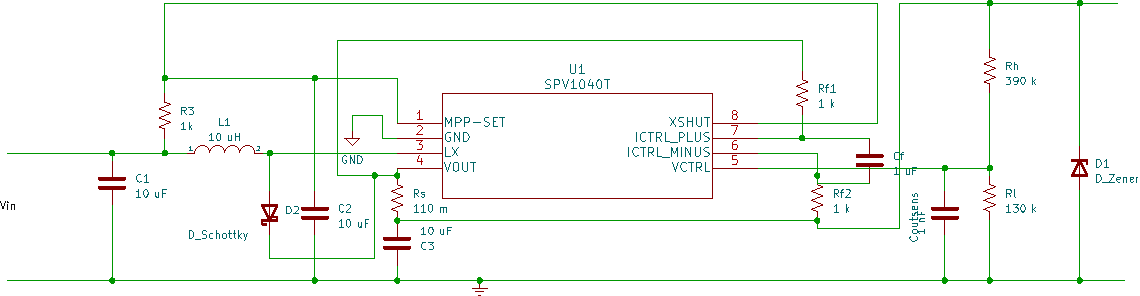
\includegraphics[width=\columnwidth]{mppt.pdf}
	\caption{MPPT circuit with SPV1040}
	\label{fig:mpptsch}
\end{figure}

\section[Battery]{Battery}
The most popular types of batteries use the following materials: Nickel Cadmium
(NiCd), Nickel Metal Hydride (NiMH), Nickel Hydrogen (NiH2), Lithium Ion
(Li-Ion) and Lithium Polymer (Li-Po). The Li-Po and Li-Ion became the standard use in space technology due to their
high energy density (Upto 200 Wh / kg on Li-Po and upto 250 Wh / kg on Li-Ion) and also due to
the number of charging cycles being as high as the NiMH, whilst presenting higher
operating temperatures. 
The Panasonic NCR 18650 GA Li-Ion cell was selected based on the calculation of EOL power, EOL efficiency and due to it's high energy density.
Specifications of Panasonic NCR 18650 GA:
\begin{itemize}
	\item Voltage: 3.7V - 4.2V
	\item Capacity: 3500mAh
	\item 1800 cycles till capacity reduces to 60\%
\end{itemize}
\section[Battery Charger]{Battery Charger}
 The battery also needs a charger to regulate its current and voltage while charging.
 BQ25302, a synchronous Buck Battery Charger IC was selected and connected in external power path mode.\\
 
 Specifications and Operating Conditions of BQ25302:
\begin{itemize}
 	\item Input Voltage: Upto 5V
 	\item Output Voltage: Upto 4.2V
 	\item Switching Frequency: 1.2MHz
 	\item Output Current: Limited to 1.2A by connecting a 33.5k resistor at ICHG pin 
 	\item Efficiency: 94.3\% at 1A from 5V input 
 	\item Thermistor: Semitec 103AT-2 (10\si{\kilo\ohm})
 	\item Charging Temperature: Limited between 0 - 45 $^{o}C$
 \end{itemize}

The Battery Charger circuit schematic is shown below:
\begin{figure}[ht]
	\centering
	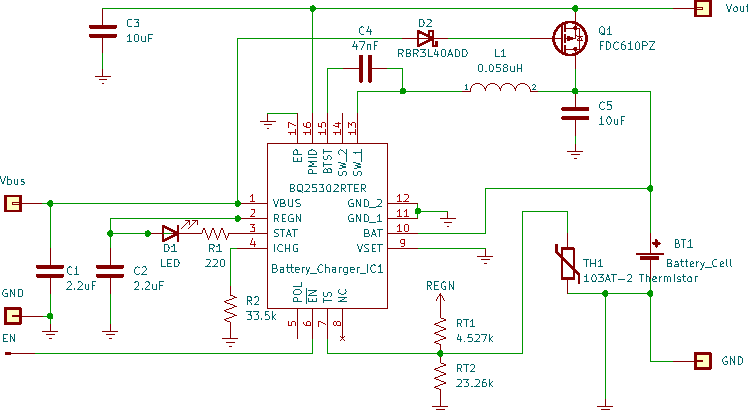
\includegraphics[width=\columnwidth]{batt2.pdf}
	\caption{Battery Charger circuit with BQ25302}
	\label{fig:battch}
\end{figure}


\section[Switching Regulators]{Buck and Boost Converters}
The power conditioning is associated with regulating the voltage to accommodate
for the charging voltage and the voltages of the satellite's subsystems. In most
subsystems, the need for a specific voltage requires a regulation of either a step-up
or a step-down of the supplied voltage. It can be done by buck
convertor(step-down) and boost converter(step-up).\\
TPS62203 was selected as the buck converter to provide step down voltage of the DC bus to supply the 3.3V loads. It is a high-efficiency synchronous step-down converter with up to 95\% efficiency.\\

 Specifications and Operating Conditions of TPS62203:
\begin{itemize}
	\item Input Voltage: 3.6 - 5V
	\item Output Voltage:  3.3V
	\item Switching Frequency: 1MHz
	\item Output Current: 300mA (max.)
\end{itemize}


 LTC3426 was selected as the boost converter to provide step up voltage of the DC bus to supply the 5V loads. It has an internal 2A MOSFET as the switch.\\
 
  Specifications and Operating Conditions of LTC3426:
 \begin{itemize}
 	\item Input Voltage: 3.6 - 5V
 	\item Output Voltage: 5V
 	\item Switching Frequency: 1.2MHz
 	\item Output Current: 500mA (max.)
 \end{itemize}
All convertors operate in continuous conduction mode.\\

The Buck and Boost Converter circuit schematic is shown below:
\begin{figure}[ht]
	\centering
	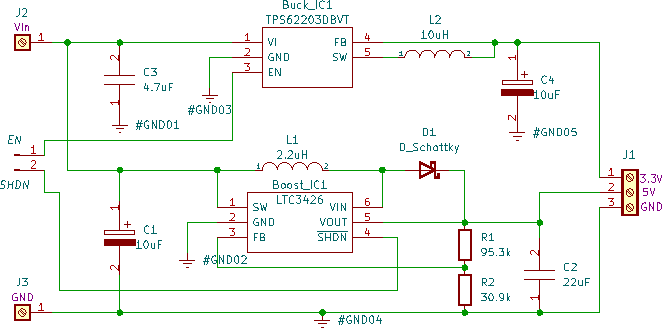
\includegraphics[width=\columnwidth]{1.pdf}
	\caption{LTC3426 as boost IC and TPS62203 as buck IC}
	\label{fig:bubo}
\end{figure}



\section[Protection Circuits]{Protection and Measurement Circuits}


LTC4361-2 is selected as the over voltage and over current protection IC. It control an external N-channel MOSFET as a switch to cut the path of current if there is an event of over current or voltage. Manual control of the MOSFET is also possible which may be useful to turn off power to buses by the micro-controller as per different modes of operation of the CubeSat.
\\

 Voltage and current passing through each bus and subsystems are continuously monitored by sensors and this information is fed to the micro-controller. These measurements help in estimation of load requirement of subsystems and also help in triggering of protection circuits if a subsystem needs to be turned off in case of an occurrence of a fault. 
 \\
 
 LTC2990 was chosen as the voltage  and current monitor. It can measure the voltage of four external channels and it's supply voltage ($V_{cc}$) simultaneously. It has a 14 bit ADC for measurement. The LTC2990 has the ability to perform 14-bit current measurements with the addition of a current sense resistor. The measurements are passed on to the micro-controller through the two wire I2C interface.
 \begin{center}
 \begin{figure}[h]
 	\centering
 	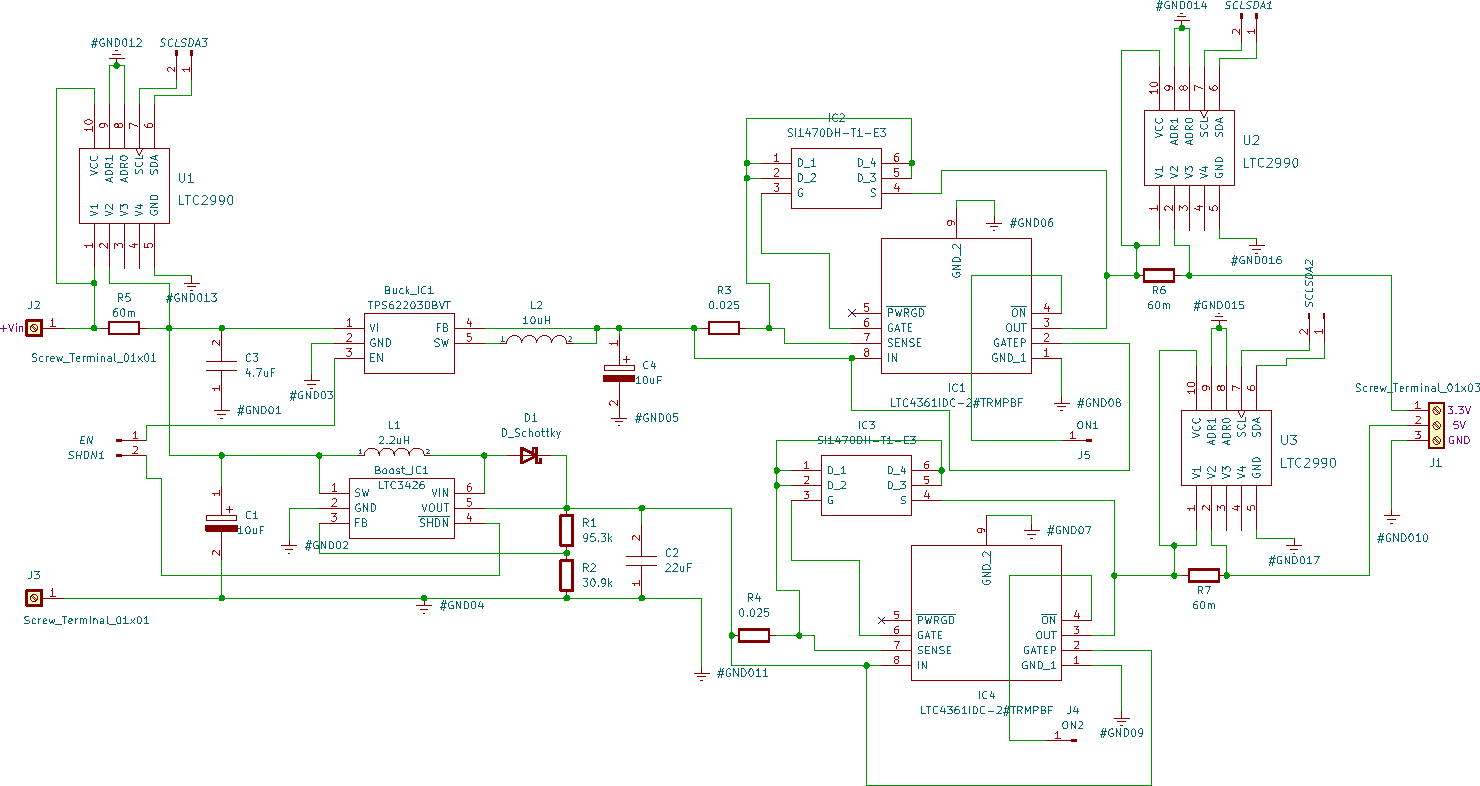
\includegraphics[width=\columnwidth]{bubowithprotn.pdf}
 	\caption{\centering Schematic of Buck and Boost circuit with Protection and Voltage and Current Measurement ICs}
 	\label{fig:bubo2}
 \end{figure}
\end{center}
The screw terminals are used to connect to the power inputs and outputs of the PCB. Pin header connectors are provided for connecting IC control pins to the micro-controller. The pin headers and their functions are given below:
 \begin{itemize}
 	\item EN pin of Buck IC: Setting LOW turns off the buck IC
 	\item SHDN pin of Boost IC: Setting LOW turns off the boost IC
 	\item ON1 pin of IC1 (LTC4361): Setting HIGH turns off the MOSFET (IC2 - SI470DH) of the 3.3V bus
 	\item ON2 pin of IC4 (LTC4361): Setting HIGH turns off the MOSFET (IC3 - SI470DH) of the 5V bus
 	\item SCLSDA1 pins: I2C connection to micro-controller relaying measured parameters of 3.3V bus by U2 (LTC2990) 
 	\item SCLSDA2 pins: I2C connection to micro-controller relaying measured parameters of 5V bus by U3 (LTC2990) 
 	\item SCLSDA3 pins: I2C connection to micro-controller relaying measured parameters of input bus ($V_{in}$) by U1 (LTC2990)
 \end{itemize}
\section{PCB Layout}
 A double layer PCB was designed from the schematic (Ref. Fig. 8.4). The second layer was used as the GROUND plane. The schematic and PCB design was done in KiCad EDA.
 
  \begin{figure}[H]
 	\centering
 	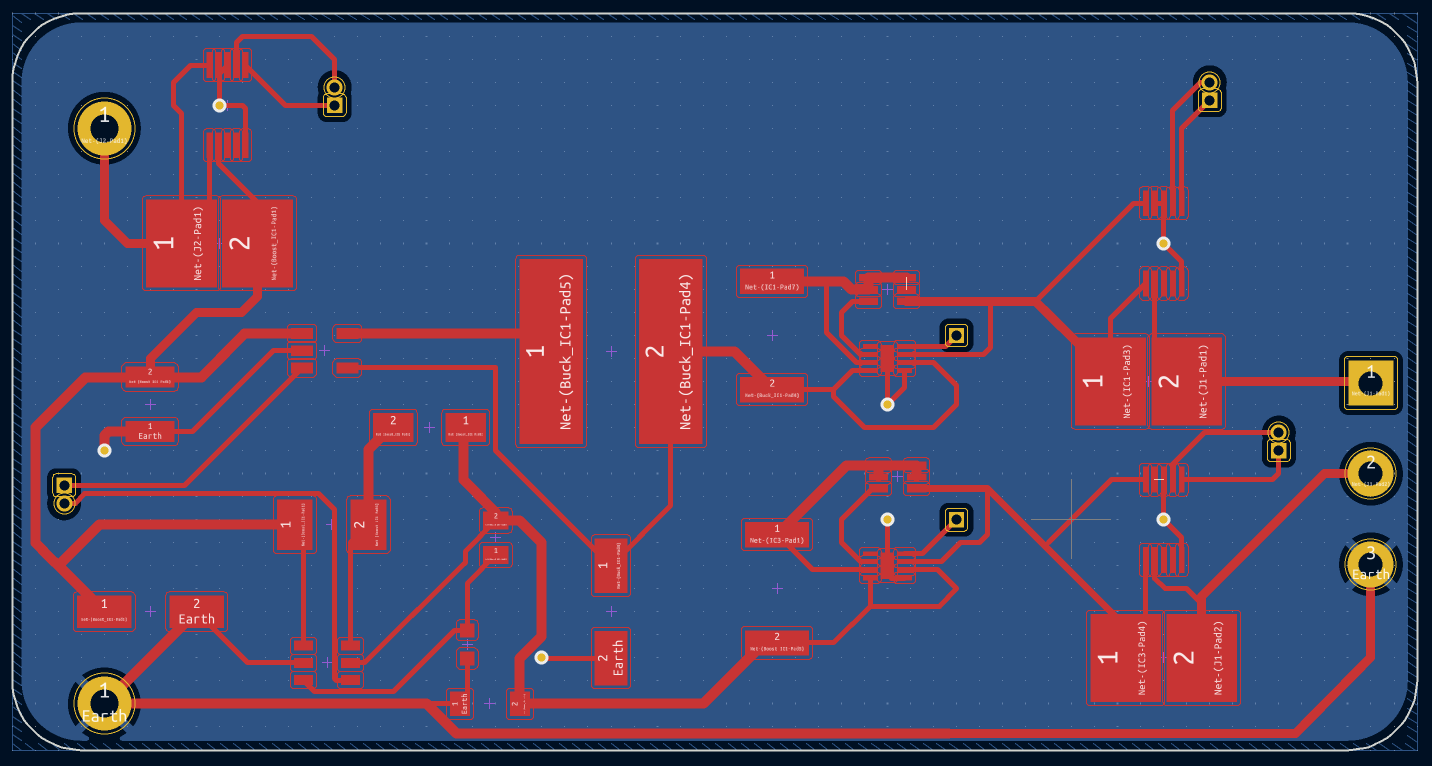
\includegraphics[width=\columnwidth]{bubopcb.png}
 	\caption{\centering Buck and Boost circuit PCB - All Copper Layers only}
 	\label{fig:bubopcb}
 \end{figure}
 
   \begin{figure}[H]
 	\centering
 	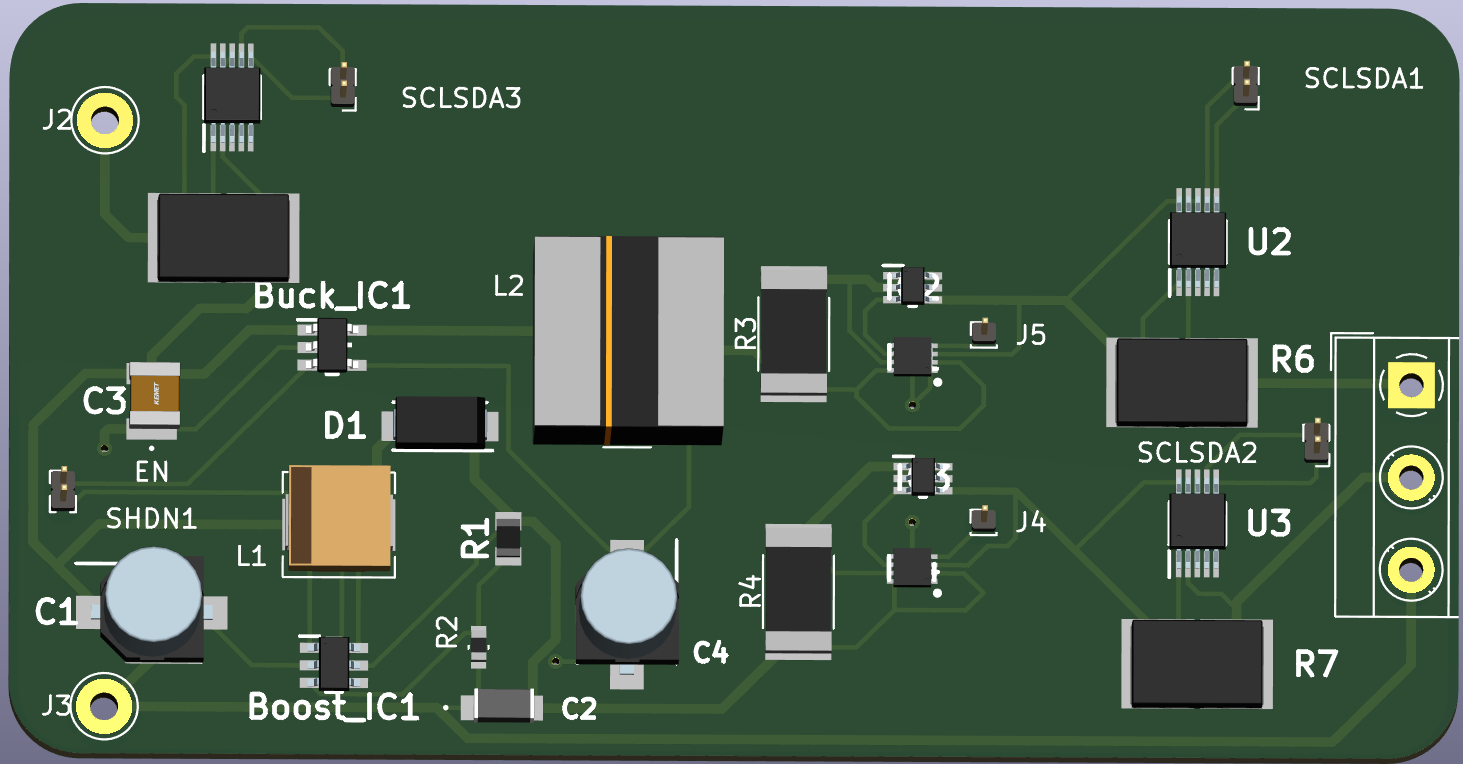
\includegraphics[width=\columnwidth]{bubopcb3d.png}
 	\caption{\centering Buck and Boost circuit PCB - 3D Model}
 	\label{fig:bubopcb3d}
 \end{figure}

\pagebreak
 \justifying
 
 \section{Micro-controller}
 The requirements of micro-controllers depend of the BUS, the other links as digital/analog outputs, the energy consumption, the voltage range and the memory.
 \\
 The micro-controller has to handle the energy distribution of the entire CubeSat, and has to communicate with the OBC of CubeSat. Thus, it needs digital/analog outputs (for lines going to ADCS, Telemetry, OBC, battery , monitoring IC etc), UART for two-way communication between the micro-controller and the OBC and SPI to  send data of the battery level to the micro-controller.
 \\
 The micro-controller should have low energy consumption, around the mirco ampere range for the “Active mode” and around the hundreds of nano ampere for the “Off mode”. It also should need sufficient memory storage to store the readings to provide it to OBC when requested. It should also independently take action during over-current, over voltage happenings, and also should control different power modes of the EPS.
 \\
 Few considered options were Arduino, Raspberry Pi, TI micro-controllers, STM32 etc. Arduino has limited programming capabilities, and Raspberry Pi was too large for the need and also has high power consumption. STM32 was selected due to its wide range of capabilities, still maintaining the size and power constraints. It also has more community support which makes the programming easier.
 \\
 STM32 is a ARM Cortex M4 32-bit micro-controller having a flash memory of 512 Kb. It can have upto 81 I/O ports with interrupt capabilities. It can have upto 78 fast I/Os upto 42 MHz, 3 I2C interfaces, 3 USARTs, 4 SPIs etc. We selected STM32401RE development board to test its capabilities, and one of its advantage is that, it can be programmed using Arduino IDE or even MATLAB, apart from its own programming IDE called STM32CUBE IDE.